% chapter 05

\chapter{Conclusions and Future Directions}\label{ch:conclusions}

\section{Ena/VASP's processive mechanism}\label{ena-mechanism-conclusions}
Initially Ena/VASP was thought to be processive only when clustered together, which was observed \textit{in vitro} with Ena/VASP clustered onto polystyrene beads \citep{breitsprecher_clustering_2008}. With the advancement of imaging technology, further observations of single molecules of Ena/VASP showed short processive runs in solution \citep{hansen_vasp_2010}. Furthermore, previous work in the Kovar lab discovered that Ena/VASP is more processive on trailing barbed ends of fascin bundles \citep{winkelman_ena/vasp_2014}. We wanted to further understand this enhanced processivity as well as Ena/VASP's underlying molecular mechanism. Our hypothesis for the enhanced processivity is that the tetrameric Ena/VASP could use its arms that were not actively adding monomer to the barbed end to bind to the sides of surrounding filaments when bound to the barbed end. This would result in the observed longer run lengths on trailing barbed ends.

With the goal of further elucidating Ena/VASP's processive molecular mechanism, we have found that Ena is more processive specifically on trailing barbed ends of fascin bundles. We saw no enhanced processivity on fimbrin or $\alpha$-actinin bundles, yet we did see enhancement with two isoforms of fascin. We also discovered that the number of Ena's arms and the number of filaments within a fascin bundle are both positively correlated with enhanced processivity on trailing barbed ends. This "avidity" effect supports our hypothesis about Ena/VASP's enhanced processivity. Furthermore, we tested two other Ena/VASP homologs, human VASP and \textit{C. elegans} UNC-34, and saw the same trend with increasing processivity with increasing fascin bundle size. We tested the effect of our oligomerization mutants, Ena\textsubscript{Dimer} and Ena\textsubscript{Trimer}, and saw that cells transfected with the mutants produced significantly less filopodia than wildtype Ena\textsubscript{Tetramer}. This result suggests that the oligomerization of Ena/VASP into tetramers is important for its function within filopodia initiation and maintenance.

\begin{figure}
\centering
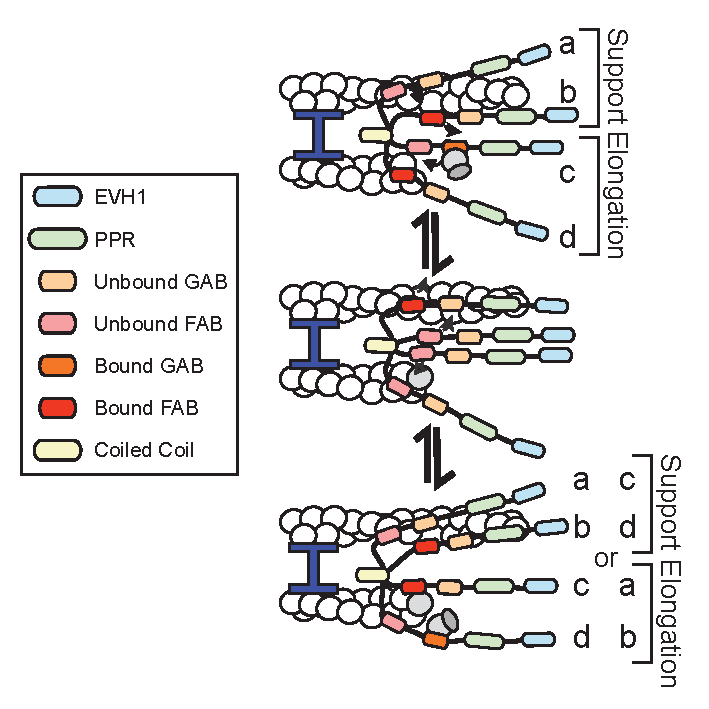
\includegraphics[width=15cm]{img/ch05/thesis_mech.pdf}
\caption[Switching arms in Ena/VASP's molecular mechanism.]{\textbf{Switching arms in Ena/VASP's molecular mechanism.} Cartoon model showing Ena/VASP adding new actin monomers on the trailing barbed end.  The cartoon shows additional arms are able to bind to the trailing or leading actin filament with the dark red FAB domains. The dark orange shows when the monomer is bound to the GAB domain. Light colored domains are unbound GAB/FAB domains.  Numbered arms show possibility of all arms being equal elongation contributors or two arms being dedicated for elongation and two arms dedicated for binding surrounding filaments. }
\label{fig:switching-mech}
\end{figure}

Ena/VASP's molecular mechanism still contains some gaps in understanding. One interesting question revolves around the role that each Ena/VASP arm plays during filament elongation. These arms could all be equal players in adding monomer as well as binding sides of filaments or certain arms could be designated for each activity (Figure \ref{fig:switching-mech}). This designation need not be by chemical modification, though that is possible in cells. Rather, it could be a random distribution of arms that initially bind either monomer or the sides of filaments, and once these arms are designated by initial binding they do not switch during that processive run. Another possibility is that the arms all fulfill each role, but they do it within the same rotation. For example, an arm could bind a monomer and this begins the process of first adding the monomer to the barbed end, then binding the elongating filament sides, then searching space for either nearby filament sides or if none are available, another actin monomer to start the process over again. Furthermore, if this is the standard process of the arms, how often interruptions to the rotation occur would be important to elucidate. This would lead to understanding the efficiency of Ena/VASP-mediated elongation.  

Another open question is whether Ena/VASP follows along the actin's helical pitch as it elongates. Formin has been shown to rotate as it processively elongates \citep{mizuno_rotational_2011}. Since both proteins processively track the barbed end, it is unclear whether rotation along the actin helix is necessary. The structural differences between formin and Ena/VASP (FH2 ring vs. four floppy arms) suggest that it would be harder for Ena/VASP to coordinate following the actin helical pitch. Additionally, since Ena/VASP is thought to cluster in cells and elongate bundled actin filaments it would not leave room for rotation of either the Ena/VASP or the actin filaments. If Ena/VASP did not need to rotate to elongate F-actin it could be one way that Ena/VASP and formin differentiate between activities in cells. However, if rotation is necessary for Ena/VASP's processive elongation it would open up many new questions on its mechanism as well as its function in cells. 

Recent studies of Ena/VASP have opened new questions about Ena/VASP tetramerization. Br\"{u}hmann et al. showed elongation and processivity are different for chimeric VASP oligomerization mutants on single filaments \citep{bruhmann_distinct_2017}. Here, we showed that processivity is positively correlated with both number of Ena arms and number of filaments in a fascin bundle. We further tested the Ena oligomerization mutants' ability to form filopodia in \textit{Drosophila} culture cells and found that they had reduced ability compared to a wildtype tetramer. These results suggest that a tetramer is better at both elongation of F-actin and staying associated with the barbed end compared to dimer and trimers. Even, \textit{in vivo} we see that the tetramer is more efficient at forming filopodia. Evolutionarily, it must have given cells an advantage to evolve tetrameric Ena/VASP over lesser oligomerization states. 

Furthermore, Br\"{u}hmann et al. showed that higher oliogmers were better than the tetramers at VASP-mediated elongation and staying associated with the barbed end on single filaments. However, there must be a reason that Ena/VASP does not form a higher oligomer. One simple argument is that producing a functional molecule from six versus four monomers puts more strain on the cell for protein production. However, with our kinetic model we also measured a proxy for Ena/VASP-mediated elongation, $\tau_{free}^{arm}$, or the time that an arm is free to bind actin monomers from solution. This measurement showed decreasing returns with higher oligomers of Ena/VASP on bundled filaments. Therefore, this is an additional explanation for why higher oligomers of Ena/VASP did not evolve. We hypothesize that an Ena/VASP tetramer lies at an ideal spot that allows for efficient elongation and processivity on F-actin, but does not require more protein production to form active molecules that are not an advantage, at least within the bundled filopodia. 

\section{Ena/VASP's role in filopodia formation}\label{ena-filopodia-conclusions}

Following the convergent elongation model of filopodia initiation \citep{svitkina_mechanism_2003}, barbed ends at the leading edge must be protected from capping protein so that these filaments can continue to elongate. Ena/VASP has been shown to compete with capping proteins for barbed ends \citep{applewhite_ena/vasp_2007,barzik_ena/vasp_2005, winkelman_ena/vasp_2014}, and having longer processive runs should also lead to better competition against capping protein during the process. Thus these filaments can then continue to grow faster through Ena/VASP-mediated elongation. Once the filaments are bundled by fascin, Ena/VASP would 'target' shorter filaments within the filopodial bundle because of its enhanced processivity on trailing barbed ends. This would protect shorter filaments in the bundle for a longer time against capping protein as well as increase their length faster through Ena/VASP-mediated elongation. Therefore, in a mature filopodia, the filaments would all be the same length and Ena/VASP would be localized to the tip.

Beyond this role of Ena/VASP for protecting trailing filaments, Ena/VASP can also be clustered in the tip complex to continue to elongate filaments. Many open questions remain about how this process works in cells, and clarifying what roles Ena/VASP plays within the process and what roles are its main function is needed. Within different cell types and even within different types of filopodia within a cell this mechanism can vary. Formin likely plays a major role within convergent elongation in most cell types so understanding how formin and Ena/VASP cooperate within this process and their concurrent regulation remains an open question. These two different types of processive polymerases are mechanistically interesting to compare and contrast to understand how different proteins maintain actin filament contact as well as how they are regulated within the cell. Understanding their individual functions as well as how they work together will give a clearer picture of what is happening at filopodia and the leading edge of the cell. Ena/VASP is also known to localize to other locations within cells such as sites of stress fiber repair and focal adhesions, but is not found to be required in these processes. It could be playing a different role at these locations since fascin bundles are not prevalent. In summary, bundling proteins could regulate actin binding proteins throughout the cell so that they preform their proper function within each actin network to which they localize. 

Though Ena/VASP has been shown to compete with capping protein, the mechanism for competition is not known. Ena/VASP is thought to occlude the barbed end by sterically blocking capping protein from binding to the barbed end. Similarly, previous genetic and biochemical work suggested that formins and capping protein were entirely antagonistic \citep{kovar_profilin-mediated_2005}. However, recent studies using single-molecule TIRFM have shown that a 'decision complex' of both capping protein and formin can be found at the barbed end. Two different formins, mDia1 and FMNL2, can form a decision complex with capping protein and it binds for a set amount of time before one protein gains sole control \citep{bombardier_single-molecule_2015,shekhar_formin_2015}. These studies open up the possibility that Ena/VASP can also share the barbed end with capping protein in another sort of decision complex. Since Ena/VASP and formin are both involved in filopodia formation and capping protein competition another open question is how the formin/capping protein decision complex responds to Ena/VASP. It is possible that Ena/VASP could help formin gain control, or even become a part of the decision complex at the barbed end. Following up these different interactions between the various barbed end binding proteins will be important for understanding processes happening at the leading edge as well as filopodia formation. 

Another notable aspect of Ena/VASP's activity is its ability to use both profilin-actin and free actin monomers to facilitate F-actin elongation. Though it is known that Ena/VASP GAB domains bind more strongly to profilin-actin than free actin monomers \citep{chereau_understanding_2006}, yet this could be a way to regulate the activity of formin-mediated filopodia formation versus Ena/VASP. Regulation by use of profilin-actin as already been shown to be a mechanism for regulating Arp2/3 complex mediated actin nucleation \citep{suarez_profilin_2015,rotty_profilin-1_2015} as Arp2/3 complex is more efficient using free actin monomers over profilin actin. Since formins are more efficient at facilitating actin elongation with profilin-actin than Ena/VASP, perhaps its when profilin-actin is low that both Arp2/3 complex and Ena/VASP activity is preferred in the cell over formin activity. Yet, since Ena/VASP is still able to use profilin-actin more efficiently, it can also cooperate with formin with both using profilin-actin. It would be interesting to measure the efficiency of profilin-actin versus free actin use by Ena/VASP and formins that are thought to bind and work together at the leading edge. In this case both proteins could use profilin-actin, but depending on the affinity and efficiency of binding profilin-actin between the two proteins, formins could predominantly use profilin-actin where Ena/VASP would be subjugated to using free-actin monomer.

\section{Regulation with actin filament bundling proteins}\label{ena-bundles-conclusions}
One major discovery in my work has been that different actin bundling proteins can regulate the binding of actin elongation factors at the barbed end of the actin filament. We found the Ena/VASP has enhanced processivity on trailing barbed ends of multiple homologs of fascin bundles, but not fimbrin or $\alpha$-actinin bundles. Though we do not yet know the mechanism behind this regulation, it suggests that all bundled networks are not created equally and this is due to a property of the bundle itself. Further support for this hypothesis is that we have shown bundling proteins intrinsically sort into domains, separating by filament spacing within their bundles. \citep{winkelman_fascin-_2016}. In this case, fimbrin and fascin sort to their narrow bundle regions while $\alpha$-actinin sorts to its own wider spaced bundled regions. In both of these situations we see differentiation of protein activity, either Ena processivity or bundler binding, due to an intrinsic property of the bundling protein forming bundles. Though this differentiation is most likely not due to the same property of the bundler since we see different sized bundlers failing to enhance Ena's processivity, these results do contribute to the possibility that bundling proteins can effect a wide range of different actin binding proteins and their dynamics within different actin networks. 

However, the mechanism of how fascin contributes to Ena's enhanced processivity on trailing barbed ends is still unknown. In our study we were able to test a few hypotheses, that fascin has a certain spacing or polarity of filaments that allows Ena to bind longer. We found that having fascin-like spacing or polarity was not sufficient to enhance Ena's processivity. Direct binding of fascin is possible, yet since Ena needs to track the barbed end of the growing trailing filament, this does not seem likely and the interaction would need to be quite weak. Additionally, there are no known Ena binding domains within fascin. Another possibility is that fascin is holding a filament in a certain twist or reducing its range of helical twist. An actin filament has a measured twist, but EM studies have shown that actin filaments actually fall within a range of degrees of twist. Fascin could reduce or shift the range of degrees that the actin can explore. One study did find that fascin has a slight rotation of the filament, but this rotation was only a single degree, which is not thought to be a large enough scale to effect actin binding proteins \citep{claessens_actin-binding_2006}. A final possibility is that fascin binds closer to the growing end of the trailing barbed end which holds the trailing barbed end closer to the side of the leading filament, allowing Ena to use the leading filament sides as additional binding sites. If fimbrin and $\alpha$-actinin allow for more flexibility of the trailing barbed end away from the leading filament, this could explain why only fascin is able to enhance Ena's processivity. Testing these different possibilities for how fascin is able to regulate Ena will give deeper understanding into Ena's molecular mechanism and also give insight into Ena's role in filopodia, as fascin is the predominant bundling protein in filopodia.

Though we have found that bundling proteins can regulate a wide variety of actin binding proteins, we have also shown that other side binding proteins can in return affect the dynamics of bundling proteins. This suggests that though bundling proteins could regulate the sorting and activity of many actin binding proteins to form different actin networks, there are still upstream actin binding proteins that could regulate the bundling proteins as well. One example that we found was that tropomyosin helps S. Pombe $\alpha$-actinin form more stable bundles. Using single-molecule TIRFM we saw that tropomyosin increases $\alpha$-actinin's dynamics on actin bundles. However, we also previously found that fimbrin can compete off tropomyosin as it bundles F-actin \citep{christensen_competition_2017}. We also recently found that fimbrin can compete off $\alpha$-actinin. However, both tropomyosin and $\alpha$-actinin can compete against fimbrin. This is a complex regulation network where tropomyosin can help one bundling while being removed by another. Interestingly both $\alpha$-actinin and fimbrin use the same CH domain to bind to actin and bind actin in the same region. How tropomyosin binding to F-actin can assist one bundling protein and be removed by another is still an open question. Our studies of different bundling proteins have shown that they can regulate different protein's localization and activity. It is important to understand how the bundling proteins are able to regulate different actin binding proteins, perhaps without any direct interaction. One possibility is that long range effects of the bundling could cause changes in other actin binding proteins. One recent study has proposed that different bundling proteins can have long range effects of the actin filament \citep{turmer_fascin_2015}. Also understanding how different actin bundling proteins are regulated by typical signaling molecules as well as other actin binding proteins will be important for understanding how different actin networks are built at certain times and locations within the cell. Targeting bundling proteins for further investigation of their effects on different actin network formation is ideal since bundling proteins can bind along the sides of actin filaments, which increases the number of binding sites as well as greatly impact an actin network's architecture.  

\section{Actin bundling proteins and their effect on convergent elongation}\label{bundler-conclusions}

Interestingly, we have found that the bundling protein that allows for longer processive runs of Ena is also the main bundling protein in the actin network that is formed of long, straight parallel bundles, filopodia. Fascin is important for filopodia formation, but may play a role beyond just forming F-actin bundles that can create force to extend the cell membrane \citep{vignjevic_role_2006,cant_drosophila_1994}. Fascin bundles within the nascent filopodia could regulate Ena/VASP to allow for increased processivity on trailing barbed ends within the bundle. This increased processivity would allow for better inhibition of capping protein and longer filaments, allowing the trailing barbed ends to catch up to the leading barbed ends. 

Moreover, another protein we've found to be regulated by fascin bundling is Arp2/3 complex, which is another player within filopodia formation via the convergent elongation model. The convergent elongation model proposes that actin filaments found in the filopodia are initially nucleated by the Arp2/3 complex. However, within the filopodia itself there is no branching of actin filaments, which raises the question of how Arp2/3 complex is inhibited along the filopodia filaments. We found that fascin bundles facilitate a decrease in Arp2/3 complex-mediated branching. Although fascin does not completely inhibit branching, it does significantly reduce Arp2/3 complex-mediated branching 2-fold. This suggests that fascin could play a role in inhibiting Arp2/3 complex, but it is not sufficient on its own to completely stop branching. Therefore, another factor must be in play to stop Arp2/3 complex from forming branches off the sides of filopodia filaments. 

Ena/VASP was shown to have anti-branching properties in early studies \citep{bear_antagonism_2002,plastino_actin_2004,samarin_how_2003, skoble_pivotal_2001}. However, recent studies have found that VASP can bind to the NPF WAVE complex and enhance Arp2/3 complex-mediated actin assembly \citep{chen_ena/vasp_2014,havrylenko_wave_2015}. Though these results seem contradictory, both of these activities could be taking place depending on the localization of Ena/VASP to the leading edge with WAVE complex, or within filopodia bundles. Further investigation is needed to understand how Ena/VASP is functioning at the leading edge and within filopodia, especially related to Arp2/3 complex.

\section{Pathogenic bacteria target the host actin cytoskeleton}\label{bacteria-conclusions}
Actin is a good target for pathogenic bacteria as the actin cytoskeleton plays many vital roles within cells. ACD toxin-mediated actin oligomers can regulate endogenous actin assembly and nucleation proteins, such as Ena/VASP and Arp2/3 complex. The oligomers bind to these proteins' actin binding domains but cannot be formed into F-actin. In the presence of the oligomers actin elongating proteins such as formin and Ena/VASP turn into capping proteins. This can be explained by either a higher affinity of the oligomers for actin binding domains or if the affinity is equal to G-actin, that the addition of free actin monomer to F-actin is the main pathway for release of actin monomers from their actin binding domains. Since the oligomers cannot be added in this situation, they remain bound to the actin binding domains. However, when observing Ena/VASP in the presence of actin oligomers it appeared that Ena/VASP bound much longer to filaments when actin assembly was stopped by the actin oligomers than during normal elongation. How the oligomer can maintain the association of Ena/VASP with the barbed end is not clear. Understanding how the oligomer is binding to Ena/VASP and affecting its assembly properties would give not only insight into the ACD toxin's mechanism but also the mechanism of Ena/VASP. Interestingly, VopL/F which are \textit{Vibrio} nucleating proteins also fall victim to ACD oligomers. The ratio of VopL/F compared to all the endogenous actin assembly proteins could be small enough that this side effect of blocking VopL/F is not apparent, yet understanding how these two processes work in tandem within cells will be important for a complete picture of \textit{Vibrio} bacteria's pathogenic mechanism. 

In our study of VopL/F we found that depending on the concentration of profilin, and such the free monomer available for nucleation, affects VopL/F's binding. With saturating profilin we still see a majority of VopL/F nucleating from the pointed end, but do see some (<15\%) molecules binding to the barbed end as well. Additionally, when no actin monomers are present VopL/F can bind to the barbed end of pre-assembled filaments for 25-30 s, which is much shorter than they stay bound to the pointed end during nucleation, 110 s. This switching of activity in the presence or absence of free actin monomer suggests that VopL/F can bind to actin monomers, profilin-actin, and F-actin. To fully understand how these molecules choose these different binding partners we must carefully measure the affinity. The TIRFM experiments suggest that VopL/F bind the strongest to actin monomers, followed by profilin-actin, and finally F-actin. VopL/F has been suggested to be structurally similar to Ena/VASP proteins and this switching of activity suggests that VopL/F's WH2 domains could act as a GAB or FAB domain. Comparing the structure and binding of Ena/VASP's GAB and FAB domain with VopL/F's WH2 domains could give an overall categorization of how WH2-like domains bind to actin differently when in different forms (i.e. G-actin, profilin-actin, F-actin). 

\section{Concluding Remarks}\label{final-conclusions}
We have further elucidated the molecular mechanism of Ena/VASP on single and bundled filaments and found that Ena/VASP has enhanced processivity specifically on trailing barbed ends of fascin bundles. This shows a novel mechanism for regulation of actin assembly proteins mediated by actin bundling proteins. We have also seen that fascin bundling can reduce Arp2/3 complex-mediated branching. Both of these fascin-mediated regulations are important for filopodia formation via the convergent elongation model. Further observations that two different bundling proteins, $\alpha$-actinin and fascin, sort to different domains due to an intrinsic spacing property adds to the importance of actin bundling proteins for regulating actin binding proteins in general. In addition, these actin bundling proteins can be regulated by other proteins as well, such as we have found with tropomyosin increasing S. Pombe $\alpha$-actinin's dynamics. These actin binding proteins are ideal targets for pathogenic bacteria and actin assembly proteins such as Ena/VASP are targeted by ACD toxin-mediated actin oligomers. Studying the actin binding proteins of the pathogenic bacteria, such as VopL/F, can give us not only insight into their disease causing mechanisms, but also how they are related to endogenous actin binding proteins. Here, I've shown that understanding how different actin binding proteins regulate other proteins' activities and affect their molecular mechanisms is a complicated goal, yet in the past years great strides have been made to understand down to a molecular level how these hundreds of proteins function to form the diverse actin networks that are necessary for vital cellular processes.

